\subsection{Resultados en la fuente S2}

\subsubsection{Análisis de Grafos}

A partir de los paquetes que se intercambian en distintas redes vemos los grafos subyacentes a las mismas. En estos cada vertice representa una IP local y cada arista va del origen al destino de un paquete who-has del protocolo ARP.

\subsubsubsection{Red Domiciliaria}

En este grafo los dos nodos con mayor grado son 192.168.1.1 con grado 7 y 192.168.1.112

\begin{figure}[H]
 \centering
	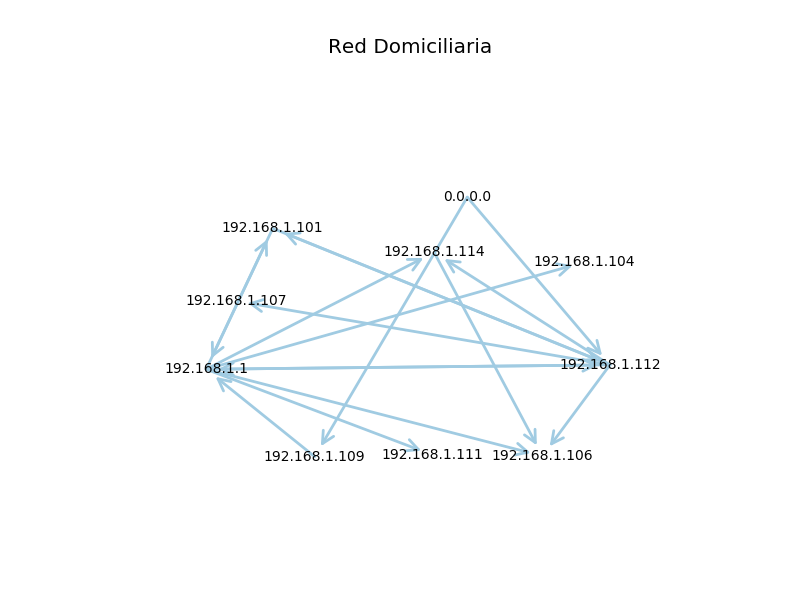
\includegraphics[width=0.8\textwidth]{figs/red_domiciliaria.png}
	\caption{}
	\label{fig:starbucks-grafo}
\end{figure}

\subsubsubsection{Starbucks}

Este grafo tiene solo dos nodos de los cuales el unico que recibe paquetes es el nodo 172.19.96.1

\begin{figure}[H]
 \centering
	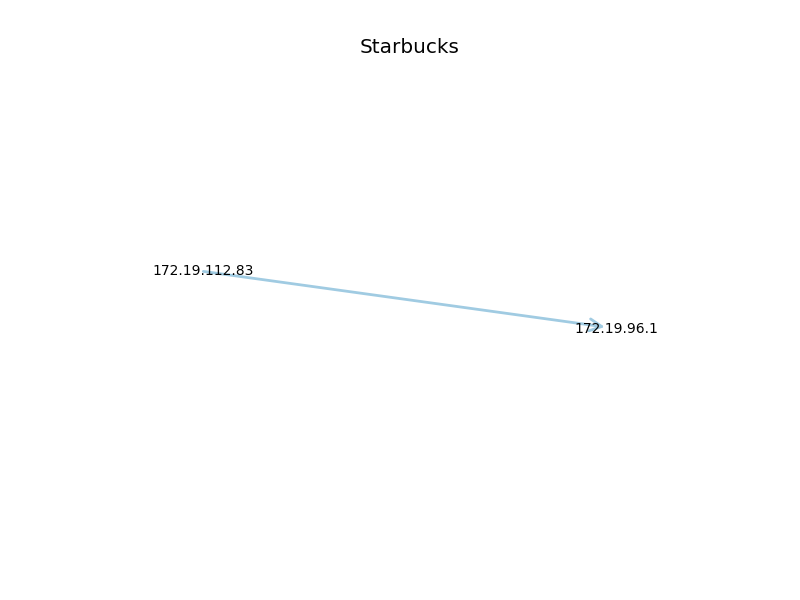
\includegraphics[width=0.8\textwidth]{figs/starbucks.png}
	\caption{}
	\label{fig:domicilio-grafo}
\end{figure}


\subsubsubsection{Laboratorios del DC}

Este grafo es mucho mas grande que los anteriores y cuenta con un nodo de maximo grado el cual es el 10.2.203.254.

\begin{figure}[H]
 \centering
	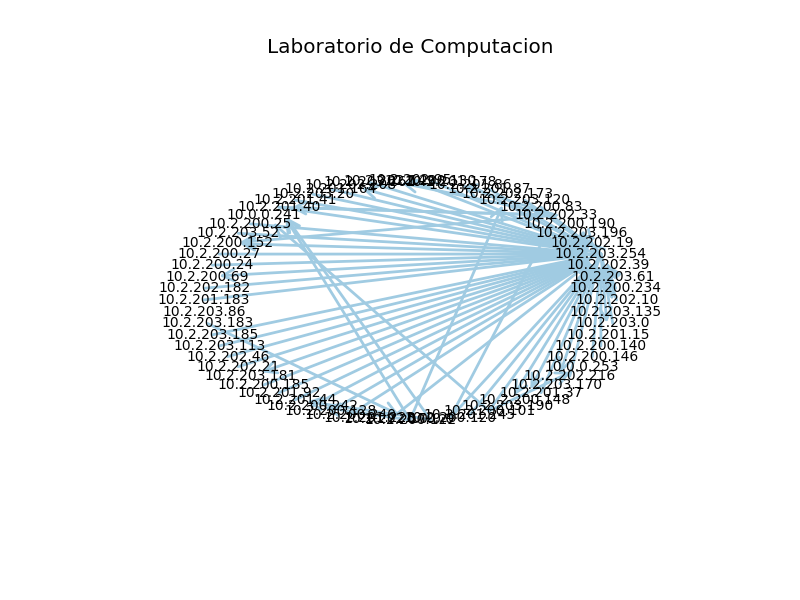
\includegraphics[width=0.8\textwidth]{figs/dc.png}
	\caption{}
	\label{fig:dc-grafo}
\end{figure}